\chapter{Introduction}\label{sec:introduction}

Jigsaw puzzles were first introduced in the 1760s when they were made from wood.  The name ``jigsaw'' derives from the jigsaws that were used to carve the wooden pieces.   The 1930s saw the introduction of the modern jigsaw puzzle where an image was printed on a cardboard sheet that was cut into a set of interlocking pieces~\cite{williams1990, williams2004}.  Although jigsaw puzzles had been solved by children for more than two centuries, it was not until 1964 that the first automated jigsaw puzzle solver was proposed by Freeman \&~Gardner~\cite{freeman1964}.  While an automated jigsaw puzzle solver may seem trivial, the problem has been shown by Altman~\cite{altman1990} and Demaine \&~Demaine~\cite{demaine2007} to be strongly NP-complete when inter-piece compatibility is not a reliable metric for determining adjacency.  

In recent years, most research into automated jigsaw puzzle solving has focused on jig swap puzzles, where all pieces are equal-sized, non-overlapping squares.\footnote{Unless otherwise noted, the phrase ``jigsaw puzzle'' is used in this thesis to refer to specifically jig swap puzzles.}  An example of a jig swap puzzle is shown in Figure~\ref{fig:jigSwapExample}.  Since all pieces are squares, shape cannot be considered when determining piece adjacency. Moreover, in this specific variant of the problem, the original, also known as ``ground-truth,'' input is not provided to the solver.  These two factors significantly increase the problem's difficulty as the complete solution's structure must be determined using only the image information on the individual pieces.

There are clear parallels between jig swap puzzle solving and other domains where an unknown object must be reconstructed from a set of component pieces.  As such, strategies developed for use with jigsaw puzzles can often be generalized to many practical problems.  Some example applications where such techniques have been applied include: reassembly of archaeological artifacts~\cite{brown2008, koller2006}, forensic analysis of deleted files~\cite{garfinkel2010}, image editing~\cite{cho2008}, shredded document reconstruction~\cite{zhu2008}, DNA fragment reassembly~\cite{marande2007}, and speech descrambling~\cite{zhao2007}. 

\begin{figure}
\centering
  \begin{tabular}{ >{\centering\arraybackslash}m{2.8in} >{\centering\arraybackslash}m{2.8in} }
	\fbox{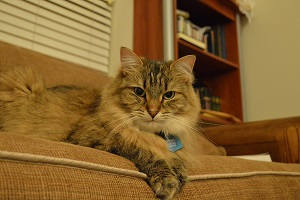
\includegraphics[width=0.365\textwidth]{./images/muffins_300x200.jpg}} & \fbox{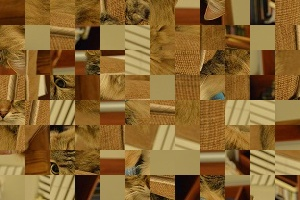
\includegraphics[width=0.365\textwidth]{./images/muffins_scrambled.jpg}}
	\\ ~\\
	(a) Ground-Truth Image & (b) Randomized Jig Swap Puzzle
	\\ ~\\
  \end{tabular}
\caption{Jig Swap Puzzle Example}
\label{fig:jigSwapExample}
\end{figure}

This thesis presents a fully-automated solver for the simultaneous assembly of multiple jigsaw puzzles, with an overview of the architecture provided in Chapter~\ref{chap:mixedBagSolver}.  Chapter~\ref{chap:quantifyingSolverQuantify} introduces a set of new metrics specifically tailored for quantifying the quality of outputs of multiple puzzle solvers; the chapter also outlines a set of standards for visualizing the characteristics of solver outputs.  Lastly, Chapter~\ref{chap:experimentalResults} compares the performance of this new solver with the current state of the art.